%%%%%%%%%%%%%%%%%%%%%%%%%%%%%%%%%%%%%%%%%%%%%%%%%%%%%%%%%%%%%%%%%%%%%%%%%%%%%%%
% Projeto para concurso público de Pesquisador Adjunto I em Sismologia.
%
% Formatação inspirada em:
% * https://github.com/leouieda/memorial2023% * https://github.com/birocoles/memos

%%%%%%%%%%%%%%%%%%%%%%%%%%%%%%%%%%%%%%%%%%%%%%%%%%%%%%%%%%%%%%%%%%%%%%%%%%%%%%%

%%%%%%%%%%%%%%%%%%%%%%%%%%%%%%%%%%%%%%%%%%%%%%%%%%%%%%%%%%%%%%%%%%%%%%%%%%%%%%%
% Set a class and import packages
\documentclass[10pt,a4paper,oneside]{book}

% Variables
\newcommand{\Year}{2024}
\newcommand{\Author}{Diogo Luiz de Oliveira Coelho}
\newcommand{\Title}{Projeto de \Author{} para concurso público - Pesquisador Adjunto I em Sismologia - ON/MCTI}
\newcommand{\Email}{diogoloc@on.br}
\newcommand{\EmailPersonal}{locdiogo@gmail.com}
\newcommand{\ORCID}{0000-0001-5426-0455}
\newcommand{\ResearchGate}{https://www.researchgate.net/profile/Diogo-De-Oliveira-Coelho}
\newcommand{\Lattes}{4330106475199471}

% Import packages
\usepackage[utf8]{inputenc}
\usepackage[T1]{fontenc}
\usepackage[brazil]{babel}
\usepackage{geometry}
\usepackage{graphicx}
\usepackage{amssymb}
\usepackage{amsmath}
\usepackage{mathpazo}
\usepackage{hyperref}
% create fancy headers
\usepackage{fancyhdr}
% commands for managing dates and its formats
\usepackage{datetime2}
% improved urls with proper hyphenation
\usepackage{xurl}
% Control over enumerate and itemize
\usepackage{enumitem}
% Tweak the look of captions
\usepackage{caption}
% To control the style of section titles
\usepackage{titlesec}
% Add the bibliography to the table of contents
\usepackage[nottoc,chapter]{tocbibind}
\usepackage[round,authoryear,sort]{natbib}
% show dois as links on references
\usepackage{doi}
% Icon and fonts (requires using xelatex or luatex)
\usepackage{fontawesome5}
\usepackage{academicons}
\usepackage{fontspec}
\usepackage[mono]{notomath}
% To make everything neater
\usepackage{microtype}
% To make fancy text boxes
\usepackage{xcolor}
\usepackage[framemethod=default]{mdframed}
% For fancy and multipage tables
\usepackage{tabularx}
\usepackage{ltablex}
% To define custom environments
\usepackage{environ}
\usepackage{setspace}
% Reference sections by name
\usepackage{nameref}
% Better handling of footnotes inside summary boxes
\usepackage{footmisc}

%to rotate the page
\usepackage{pdflscape}

%To plot piechart
\usepackage{bera}
\usepackage{pstricks-add}
\usepackage{pgf-pie}

\usepackage{wrapfig}

%%%%%%%%%%%%%%%%%%%%%%%%%%%%%%%%%%%%%%%%%%%%%%%%%%%%%%%%%%%%%%%%%%%%%%%%%%%%%%%

%%%%%%%%%%%%%%%%%%%%%%%%%%%%%%%%%%%%%%%%%%%%%%%%%%%%%%%%%%%%%%%%%%%%%%%%%%%%%%%
% Configuration of the document

\geometry{%
  left=30mm,
  right=30mm,
  top=20mm,
  bottom=15mm,
  headsep=5mm,
  headheight=5mm,
  footskip=10mm,
  includehead=true,
  includefoot=true
}

% Increase the line spacing
\SetSinglespace{1.2}
\onehalfspacing

% Remove spacing between enumerate/itemize items
\setlist{nosep}

% Padding between the first figure and the chapter title
\newcommand{\HeroFigPad}{\vspace{-1cm}}

% Padding before the software logo figures
\newcommand{\SoftwareFigPad}{\vspace{-0.3cm}}

% Add a link to a DOI
\newcommand{\DOI}[1]{\url{https://doi.org/#1}}

% Add a link to a GitHub repository
\newcommand{\GitHub}[1]{\faGithub{} Código: \url{https://github.com/#1}}

% Add a link to a YouTube video
\newcommand{\YouTube}[1]{\faYoutube{} Vídeo: \url{https://youtu.be/#1}}

% Add a link to a supplementary data
\newcommand{\Data}[1]{\faChartBar{} Dados: \url{https://doi.org/#1}}

% Add a link to a preprint
\newcommand{\Preprint}[1]{\faLockOpen{} Preprint: \url{https://doi.org/#1}}

% Make a Unicode bullet symbol
\newcommand{\Bullet}{•\enspace}

% Define custom colors
\definecolor{lu_gray}{gray}{0.98}
\definecolor{lu_darkgray}{gray}{0.3}
\definecolor{gold(metallic)}{rgb}{0.83, 0.69, 0.22}
\definecolor{cornsilk}{rgb}{1.0, 0.97, 0.86}
\definecolor{lu_blue}{RGB}{32, 96, 194}
\definecolor{lu_lightblue}{RGB}{238, 245, 250}
\definecolor{timberwolf}{rgb}{0.86, 0.84, 0.82}
\definecolor{battleshipgrey}{rgb}{0.52, 0.52, 0.51}

% Customize how Chapter headings are displayed
\titleformat{\chapter}[display]{\normalfont}{\large Capítulo \thechapter}{0pt}{\huge}[\titlerule]
\titlespacing*{\chapter}{0pt}{-40pt}{40pt}

% Set the spacing between bibliography entries (requires natbib)
\setlength{\bibsep}{0pt}

% Configure captions
\captionsetup{labelfont=bf,font={small,color=lu_darkgray},skip=0pt}

% Define a fancy text for summarybox
\mdfdefinestyle{summarybox}{%
  leftline=true,
  rightline=false,
  topline=false,
  bottomline=false,
  linewidth=4pt,
  linecolor=gold(metallic),
  frametitlefont=\bfseries\color{black}\small,
  frametitlebackgroundcolor=cornsilk,
  frametitleaboveskip=7pt,
  frametitlebelowskip=7pt,
  frametitlerule=true,
  frametitlerulewidth=1pt,
  backgroundcolor=lu_gray,
  innertopmargin=7pt,
  innerbottommargin=10pt,
  innerleftmargin=15pt,
  innerrightmargin=15pt,
  skipbelow=5pt,
  skipabove=0pt,
}
\newmdenv[style=summarybox]{summarybox}

% Define a fancy text for subsummarybox
\mdfdefinestyle{subsummarybox}{%
  leftline=true,
  rightline=false,
  topline=false,
  bottomline=false,
  linewidth=4pt,
  linecolor=battleshipgrey,
  frametitlefont=\bfseries\color{black}\small,
  frametitlebackgroundcolor=timberwolf,
  frametitleaboveskip=7pt,
  frametitlebelowskip=7pt,
  frametitlerule=true,
  frametitlerulewidth=1pt,
  backgroundcolor=lu_gray,
  innertopmargin=7pt,
  innerbottommargin=10pt,
  innerleftmargin=15pt,
  innerrightmargin=15pt,
  skipbelow=5pt,
  skipabove=0pt,
}
\newmdenv[style=subsummarybox]{subsummarybox}

% Define a fancy text for projectbox
\mdfdefinestyle{projectbox}{%
  leftline=true,
  rightline=false,
  topline=false,
  bottomline=false,
  linewidth=4pt,
  linecolor=lu_blue,
  frametitlefont=\bfseries\color{black}\small,
  frametitlebackgroundcolor=lu_lightblue,
  frametitleaboveskip=7pt,
  frametitlebelowskip=7pt,
  frametitlerule=true,
  frametitlerulewidth=1pt,
  backgroundcolor=lu_gray,
  innertopmargin=7pt,
  innerbottommargin=10pt,
  innerleftmargin=15pt,
  innerrightmargin=15pt,
  skipbelow=5pt,
  skipabove=0pt,
}
\newmdenv[style=projectbox]{projectbox}

% Define something like an fa-ul and a date list
\NewEnviron{fa-ul}{%
  \vspace{-0.4cm}
  \small
  \renewcommand{\arraystretch}{1.25}
  \begin{tabularx}{\linewidth}{@{}p{0.05\linewidth}@{}@{}p{0.95\linewidth}@{}}
    \BODY
  \end{tabularx}%
}
\NewEnviron{datelist}{%
  \vspace{-0.4cm}
  \small
  \renewcommand{\arraystretch}{1.25}
  \begin{tabularx}{\linewidth}{@{}p{0.15\linewidth}@{}@{}p{0.85\linewidth}@{}}
    \BODY
  \end{tabularx}%
}
\NewEnviron{paperlist}{%
  \vspace{-0.4cm}
  \small
  \renewcommand{\arraystretch}{1.25}
  \begin{tabularx}{\linewidth}{@{}p{0.08\linewidth}@{}@{}p{0.92\linewidth}@{}}
    \BODY
  \end{tabularx}%
}
\NewEnviron{courselist}{%
  \vspace{-0.4cm}
  \small
  \renewcommand{\arraystretch}{1.25}
  \begin{tabularx}{\linewidth}{@{}p{0.15\linewidth}@{}@{}p{0.85\linewidth}@{}}
    \BODY
  \end{tabularx}
}

% Define a fancy enumerate that has a title
\NewEnviron{fancyenum}[2]{%
  \vspace{0.25cm}
  \noindent#1\quad\textbf{#2}:
  \vspace{0.25cm}
  \begin{enumerate}
    \BODY
  \end{enumerate}
}

% Configure hyperref and add PDF metadata
\hypersetup{
    colorlinks,
    allcolors=lu_blue,
    pdftitle={\Title},
    pdfauthor={\Author},
    pdftex,
    breaklinks=true,
}

% make urls use the same font as every other text
\urlstyle{same}

% Prevent footnotes from being broken into multiple pages
\interfootnotelinepenalty=10000

% Configure headers and footers
\fancyhf{}
\lhead{\fontsize{9pt}{0}\selectfont\itshape \nouppercase\leftmark}
\chead{}
\rhead{\fontsize{9pt}{0}\selectfont \thepage}
\cfoot{}
\renewcommand{\headrulewidth}{0.3pt}
%%%%%%%%%%%%%%%%%%%%%%%%%%%%%%%%%%%%%%%%%%%%%%%%%%%%%%%%%%%%%%%%%%%%%%%%%%%%%%%

%%%%%%%%%%%%%%%%%%%%%%%%%%%%%%%%%%%%%%%%%%%%%%%%%%%%%%%%%%%%%%%%%%%%%%%%%%%%%%%
\begin{document}

\pagestyle{plain}
\frontmatter

\begin{titlepage}
  \begin{center}
    \includegraphics[height=2cm]{images/logo_terra.png}
    \vspace{1cm}

    CONCURSO PÚBLICO
    
    PESQUISADOR ADJUNTO I EM SISMOLOGIA
    
    OBSERVATÓRIO NACIONAL

    \vspace{5cm}

    \textbf{\LARGE Proposta de projeto de pesquisa}
    \vspace{1cm}

    \textbf{\LARGE \MakeUppercase{\Author{}}}
    \vspace{5cm}

    {\small
	Apresentado para concurso público de provas e títulos para cargo de

	Pesquisador Adjunto I em Sismologia do Observatório Nacional.
      \vspace{1cm}

	EDITAL N$^{\circ}$   1, DE 9 DE OUTUBRO DE 2023
    }
    \vfill

    \Year{}
  \end{center}
\end{titlepage}

%==============================================================================
\chapter*{Resumo}

A presente proposta de projeto de pesquisa representa um esforço dedicado à investigação e avanço de áreas da sismologia brasileira, principalmente quando se refere à parte acústica e hidroacústica. Este projeto tem como objetivo preencher lacunas identificadas previamente, visando a ampliação e aprofundamento da compreensão nesses temas desafiadores, que possuem grande potencial para trabalhos interdisciplinares. Com base na revisão da literatura e na identificação de questões ainda não exploradas, esta proposta visa desenvolver uma série de estudos inovadores que possam agregar valor teórico e prático à comunidade científica, além de aumentar a área de contato com temas relevantes para a sociedade civil. Com uma abordagem interdisciplinar, o projeto visa não apenas responder a perguntas específicas de pesquisa, mas também promover o diálogo interdisciplinar e a colaboração entre diferentes áreas de conhecimento relacionadas aos diversos temas abordados. No momento, as principais áreas do conhecimento em geociências que essa proposta de projeto visa abordar são: geofísica, geologia, oceanografia e meteorologia.  

\begin{landscape}
% Conteúdo da página em modo paisagem
\begin{figure}[tb]
\begin{center}
\includegraphics[width=\pagewidth]{images/linha_do_projeto.png}
\end{center}
\caption*{Resumo cronológico dos temas a serem desenvolvidos. Borda completa: plena capacidade de desenvolvimento e experiência prática, Borda incompleta: necessidade de aperfeiçoamento de metodologias e experiência prática incompleta, Borda tracejada: falta de arcabouço teórico e prático.}
\label{fig_tempo_linha}
\end{figure}
\end{landscape}
%==============================================================================
\tableofcontents

\mainmatter
\pagestyle{fancy}

%==============================================================================
\chapter{Apresentação}

\begin{minipage}[b]{0.5\linewidth}
{\faUser} \textbf{Identificação:} Diogo Luiz de Oliveira Coelho\\
{\faIcon{at}} \textbf{e-mail profissional:}  \href{mailto:\Email}{\Email} \\
{\faIcon{at}} \textbf{e-mail pessoal:}  \href{mailto:\EmailPersonal}{\EmailPersonal}\\
\textbf{Links úteis: }  
\href{https://orcid.org/\ORCID}{\Large \aiOrcid}
\href{\ResearchGate}{\Large \aiResearchGate}
\href{https://lattes.cnpq.br/\Lattes}{\Large \aiLattes}
\href{https://github.com/diogoloc}{\Large \faIcon{github}}
\end{minipage}
\begin{minipage}[b]{0.5\linewidth}
\centering
\includegraphics[scale=0.1]{images/foto.jpg}
\end{minipage}

\bigskip	
\bigskip	
\bigskip	
\bigskip	

\begin{summarybox}[frametitle=\faAward{}\quad Resumo da formação e atuação acadêmica]
  \begin{datelist}
    2007--2012 & Bacharelado em Geologia (UFES) \\
    2013--2015 & Mestrado em Geofísica (ON) \\
    2015--2019 & Doutorado em Geodinâmica e Geofísica (UFRN) \\
    2020--2021 & Estágio Pós-doutoral I (UFSC) \\
    2022--2023 & Estágio Pós-doutoral II  (ON) \\
    2023--atual & Estágio Pós-doutoral III (ON)
  \end{datelist}
\end{summarybox}

\bigskip	

Durante a confecção desta proposta, vislumbrei não apenas ampliar, mas também aprofundar o escopo das atividades do Observatório Nacional no campo da Sismologia em consonância com questões globalmente relevantes. O foco principal é o desenvolvimento de iniciativas que ofereçam resultados práticos para a demandas atuais da Sismologia do Observatório Nacional e também atender às necessidades contemporâneas da sociedade civil. Como exemplo, posso citar o monitoramento de potenciais fontes de desastres (naturais/antrópicos) através da análise e da divulgação de dados sobre a sismicidade brasileira. Além disso, a proposta tem como meta disponibilizar técnicas e dados de forma mais acessível e acertiva, maximizando seu uso pela sociedade e pela indústria. Este enfoque estratégico não apenas fortalece o papel do Observatório Nacional como uma instituição de referência em na Geofísica, mas também contribui significativamente para o avanço do conhecimento científico aplicado.

%==============================================================================

\chapter{Estrutura do Projeto}
\label{cap_estrutura}

\begin{figure}[h]
	\HeroFigPad
	\begin{center}
		\includegraphics[width=\textwidth]{images/arpoador.jpg}
	\end{center}
	\caption{
	O pôr do sol no \href{https://pt.wikipedia.org/wiki/Arpoador}{Arpoador} serviu de inspiração para a concepção deste Projeto de Pesquisa, uma vez que representa um espetáculo fenomenal que une o céu, o mar e a terra.
    }
 \label{fig_arpoador}
\end{figure}

Como o Projeto de pesquisa possui várias frentes de atuação em ambientes distintos. Para facilitar a leitura e o acopanhamento dos projetos de pesquisa propostos, estruturei o plano em três capítulos diferentes, cada um associado com um elemento da Figura \ref{fig_arpoador}, Mar (capítulo \ref{cap_mar}), Terra (capítulo \ref{cap_terra}) e Céu (capítulo \ref{cap_ceu}), além de posicionar cronologicamente os ambientes e projetos.

\bigskip

\begin{summarybox}[frametitle=\faStreetView{}\quad Panorama cronológico dos temas propostos]
  \begin{datelist}
    2024--2028 & Monitoramento sísmico e hidroacústico (MAR) \\
    2024--2028 & Ilhas oceânicas (MAR) \\
    2025--2030 & Estrutura profunda do Brasil (TERRA) \\
    2028--2034 & Monitoramento de barragens (TERRA) \\
    2034--2040 & Monitoramento infrassônico (CÉU) 
  \end{datelist}
\end{summarybox}

\bigskip

Observando o resumo cronológico inicial da minha proposta, é possível identificar uma sequência de temas prospostos com diferentes prazos de implementação. Esses períodos evidenciam lacunas acadêmicas, metodológicas ou práticas, por parte do autor. Por exemplo, considerando o caso do monitoramento com o uso de equipamentos de infrassom, até o momento não possuo experiência prática com esse tipo de dado. Por essa razão, na linha do tempo, ele é o último tema a ser iniciado. No entanto, como descreverei no plano de implementação (capítulo \ref{cap_ceu}), essa falta de experiência pode ser sanada através de um cronograma estruturado de ações para aumentar a minha experiência neste tema. Notadamente observa-se um alinhamento cronológico com a \href{http://www.finep.gov.br/images/contratos-Adm/2022/dou/Y_S_dias_extrato_contrato.pdf}{expansão para o mar da Rede Sismográfica Brasileira} e os projetos aqui propostos. Pois, além de participar do grupo de execução dessa expansão, eu tenho experiências com esse tipo de dados e tenho plena convicção da necessidade de implementação de novas frentes de trabalho para enfrentar os desafios desse tipo de projeto.

Nem todos os temas de projetos exemplificados nesta proposta estão em fase embrionária. Por exemplo, o tema que visa estudar as Ilhas oceânicas, já está sendo executado e já tem resultados promissores, com mostra o trabalho apresentado no 18$^\circ$ Congresso Internacional da Sociedade Brasileira de Geofísica\footnote{Resumo (2023): 18th International Congress of the Brazilian Geophysical Society, Rio de Janeiro, Brazil. \href{https://sbgf.org.br/mysbgf/eventos/expanded_abstracts/18th_CISBGf/57aeee35c98205091e18d1140e9f38cfShort_Abstract_18th_CISBGf_.docx}{Comparison of the shallow and deep structure beneath the Abrolhos Archipelago and the Trindade Island with passive-source seismology}. Eveline Sayao, Diogo Luiz de Oliveira Coelho, Daniele Ingredy Gomes Silva, Carlos Ribeiro, Sergio Luiz Fontes, Thiago Santanna, Elisabeth Lima, Ronaldo Marins}. Outro tema que já está estruturado é o Estruturua profunda do Brasil, onde já formamos um grupo de pesquisa com pesquisadores e alunos de algumas universidade para atualizar metodologias e propor ideias de trabalhos para estudar a estrutura profunda de certas áreas do Brasil com dados da \href{http://rsbr.on.br/}{RSBR}, como será exemplificado no capítulo \ref{cap_terra}. 

Para facilitar o acompanhamento das várias propostas de projetos de pesquisa, cada um dos projetos foram estruturados segundo a tabela abaixo, onde todos os projetos possuem um título, justificativa, banco de dados, objetivos,  plano de implementação, produtos e bibliografia. Ao final do documento, no capítulo \ref{cap_financiamento}, eu faço considerações sobre o tipo e a necessidade de financiamento para os projetos propostos neste documento. Por fim, minhas considerações finais sobre a proposta apresentada no capítulo \ref{cap_conclusao}.

\bigskip

\begin{subsummarybox}[frametitle=\faBullhorn\quad Constituição de cada projeto]
  \begin{fa-ul}
    \faTag & \textbf{Título:} Tema do projeto \\
    \faPencil* &  \textbf{Justificativa:} Relevância da pesquisa \\
	\faDatabase & \textbf{Banco de Dados:} Referência do banco de dados utilizado \\
    \faFutbol & \textbf{Objetivos:} Tópicos o que se pretende pesquisar \\
    \faBrain & \textbf{Plano de Implementação:} Etapas de como realizar a pesquisa  \\
    \faShoppingCart & \textbf{Produtos:} Lista com os principais resultados do projeto \\
    \faBook & \textbf{Bibliografia básica:} Referências de trabalhos fundamentais
  \end{fa-ul}
\end{subsummarybox}

%==============================================================================

\chapter{Mar}
\label{cap_mar}

\begin{figure}[h]
	\HeroFigPad
	\begin{center}
		\includegraphics[width=\textwidth]{images/obs_foto.jpeg}
	\end{center}
	\caption{
	Processo de instalação de um Sismômetro de Fundo Ocêanico no \href{https://sismo-oceano.ufsc.br/}{Projeto Monitoramento Sismo-Oceanográfico}.
    }
 \label{fig_obs}
\end{figure}

Neste capítulo, apresento de forma resumida propostas de projetos utilizando dados oriundos de áreas oceânicas.   

\section{Tema: Monitoramento Sísmico e Hidroacústico}

Como demonstrado no memorial, eu tenho experiência no processamento de banco de dados sísmicos e acústicos orindos de equipamentos oceânicos, como: sismômetros de fundo oceânico (\href{https://en.wikipedia.org/wiki/Ocean-bottom_seismometer}{OBS}), sismógrafos flutuantes (\href{https://www.geoazur.fr/GLOBALSEIS/Mermaid.html}{MERMAID}) e planadores oceânicos (\href{https://oceanservice.noaa.gov/facts/ocean-gliders.html}{GLIDER}). Após a análise desses banco de dados, sugere-se um projeto que tenha foco em metodologias de redução/supressão de ruído nos dados.

\subsection{Projeto: Redução de ruído em dados sísmicos e acústicos}

A proposta de redução de ruído se faz necessária devido ao alto nível de ruído basal encontrado globalmente em dados de equipamentos localizados em áreas oceânicas (Bayrakci \& Klingelhoefer, 2024). Devido alta sensibilidade de Sismômetros de Fundo Oceânico (OBS), o nível de ruído nesses dados é bem elevado devido a várias condicionantes (e.g. correntes de fundo oceânico, baixo acoplamento entre o sensor e o assoalho oceânico, operações submarinas próximas, etc). Existem metodologias recentes, como o trabalho de Zali et al. (2023), para a redução de ruído nos dados de OBS através de algoritmos de processamento de áudio, onde os resultados encontrados são bem satisfatórios. Para dados acústicos, temos o trabalho de Shen et al. (2024) que mostra observações de ondas T de terremotos distantes e regionais e um esquema de supressão de ruído por Curvelet para aprimorar os sinais de ondas T. No entanto, nossa ideia não é utilizar somente a transformada Curvelet, e sim utilizar a combinação das transformadas de Wavelet e Curvelet para lidar com as fraquezas individuais de cada método e suprimir ruído dos dados, como mostra Bal et al.(2019) a remoção de ruído nas imagens de Tomografia por Emissão de Pósitrons (PET).

\begin{fancyenum}{\faDatabase}{Banco de Dados}
	\item Sismômetros de Fundo Oceânico: \href{https://sismo-oceano.ufsc.br/}{Bacia de Campos e Santos} (\faLock);
	\item Planadores Submarinos: \href{https://comunicabaciadesantos.petrobras.com.br/projeto-de-monitoramento-da-paisagem-acustica-submarina-pmpas-}{Bacia de Santos} (\faLock);
	\item Hidrofones acoplados em linhas de fundeio: \href{https://comunicabaciadesantos.petrobras.com.br/projeto-de-monitoramento-da-paisagem-acustica-submarina-pmpas-}{Bacia de Santos} (\faLock);
	\item Sismógrafos flutuantes: \href{https://www.geoazur.fr/GLOBALSEIS/Data.html}{Ilha de Galápagos} (\faUnlock).
	\item Hidrofones do \href{https://www.ctbto.org/our-work/international-monitoring-system}{Sistema de Monitoramento Internacional}: \href{https://ds.iris.edu/gmap/\#network=IM\&planet=earth}{Incorporated Research Institution for Seismology} (\faUnlock);

\end{fancyenum}

\begin{fancyenum}{\faFutbol}{Objetivos}
	\item Aplicar métodos de processamento de áudio para remoção de ruído em dados sísmicos;
	\item Aplicar métodos de processamento de imagem para remoção de ruído em dados acústicos;
	\item Combinar as transformadas de Wavelet e Curvelet para aprimorar os sinais das \href{https://insu.hal.science/insu-00915042/document}{ondas T} nos dados acústicos.
\end{fancyenum}

\begin{fancyenum}{\faBrain}{Plano de Implementação}
	\item Compilação dos dados acústicos e sísmicos disponíveis;
	\item Compilação de pacotes eficientes em python para o desenvolvimento dos algoritmos computacionais;
	\item Testes com sintéticos utilizando \href{https://pyrocko.org/docs/current/apps/fomosto/tutorial.html}{FOMOSTO} e \href{https://ds.iris.edu/ds/products/syngine/}{SYNGINE}, ferramentas que fornecem acesso a sismogramas de acordo com funções de Green e modelos de Terra pré-calculados;
	\item Testes em dados reais;
	\item Elaboração de documentação do pacote computacional e dos algoritmos desenvolvidos.
\end{fancyenum}

\begin{fancyenum}{\faShoppingCart}{Produtos}
	\item Desenvolvimento de algoritmos computacionais para a remoção de ruídos em dados sísmicos e acústicos;
	\item Implementação de pacote computacional em python para compilar os algoritmos criados.
\end{fancyenum}

\begin{fancyenum}{\faBook}{Bibliografia básica}
	\item Bal, A., Banerjee, M., Sharma, P. et al. 2019. An efficient wavelet and curvelet-based PET image denoising technique. Med Biol Eng Comput 57, 2567–2598. https://doi.org/10.1007/s11517-019-02014-w;
	\item Bayrakci, G. and Klingelhoefer, F. 2024. eds. Noisy Oceans. Geophysical Monograph Series. Wiley, 28 February 2024. https://doi.org/10.1002/9781119750925;
	\item Shen, Z., \& Wu, W. 2024. Ocean bottom distributed acoustic sensing for oceanic seismicity detection and seismic ocean thermometry. Journal of Geophysical Research: Solid Earth, 129,e2023JB027799. https://doi.org/10.1029/
2023JB027799;
	\item Zali, Z., Rein, T., Krüger, F., Ohrnberger, M., and Scherbaum, F. 2023. Ocean bottom seismometer (OBS) noise reduction from horizontal and vertical components using harmonic–percussive separation algorithms, Solid Earth, 14, 181–195, https://doi.org/10.5194/se-14-181-2023.
\end{fancyenum}

\subsection{Projeto: Localização de eventos sísmicos utilizando reflexões hidroacústicas}

Eventos de grande amplitude, como explosões e terremotos, produzem sinais hidroacústicos de grande amplitude que têm sido estudados desde a Segunda Guerra Mundial. Upton et al. (2006) mostra que quando o som viaja na coluna d'água e encontra uma mudança na impedância, como um monte submarino, uma ilha ou uma plataforma continental, parte da energia pode ser dispersada ou refletida. Como relata Hanson \& Bowman (2006), é notável a eficiência da propagação hidroacústica nos oceanos. As reflexões hidroacústicas oriundas de grandes alvos batimétricos podem ser usadas para restringir as localizações de eventos quando a cobertura da estação não é ideal. Dados hidroacústicos históricos e contemporâneos de muitas explosões subaquáticas e terremotos sub-marinhos mostram grandes reflexões chegando aos receptores dezenas de minutos ou horas após a chegada direta (Upton et al., 2006). Devido a isso, o objetivo deste estudo é investigar a possibilidade de melhorar/localizar eventos hidroacústicos locais registrados por hidrofones instalados na costa sudeste do Brasil. 

\begin{fancyenum}{\faDatabase}{Banco de Dados}
	\item Hidrofones acoplados em OBS: \href{https://sismo-oceano.ufsc.br/}{Bacia de Campos e Santos} (\faLock);
	\item Hidrofones acoplados em linhas de fundeio: \href{https://comunicabaciadesantos.petrobras.com.br/projeto-de-monitoramento-da-paisagem-acustica-submarina-pmpas-}{Bacia de Santos} (\faLock);
	\item Planadores Submarinos: \href{https://comunicabaciadesantos.petrobras.com.br/projeto-de-monitoramento-da-paisagem-acustica-submarina-pmpas-}{Bacia de Santos} (\faLock).
	\item Hidrofones do \href{https://www.ctbto.org/our-work/international-monitoring-system}{Sistema de Monitoramento Internacional}: \href{https://ds.iris.edu/gmap/\#network=IM\&planet=earth}{Incorporated Research Institution for Seismology} (\faUnlock);
\end{fancyenum}

\begin{fancyenum}{\faFutbol}{Objetivos}
	\item Identificar as reflexões hidroacústicas de grandes eventos sísmicos locais;
	\item Identificar as principais feições batimétricas que podem ser potencias fontes de reflexões hidroacústicas;
	\item Avaliar a viabilidade do uso de reflexões hidroacústicas para localizar eventos sísmicos locais;
	\item Estender o potencial de cobertura de detecção e localização da Rede Sismográfica Brasileira.
\end{fancyenum}

\begin{fancyenum}{\faBrain}{Plano de Implementação}
	\item Idenficação de potenciais sinais refletidos em sismogramas;
	\item Associação destes eventos com as feiçõess batimétricas proeminentes que podem atuar como superfícies refletoras;
	\item O tempo de viagem entre o refletor e o sensor é previsto usando um modelo de velocidade do som oceânico dependente da estação;
	\item As chegadas diretas e refletidas são então usadas como entrada para o algoritmo de localização padrão, conforme descrito acima.
\end{fancyenum}

\begin{fancyenum}{\faShoppingCart}{Produtos}
	\item Melhoramento da determinação da localização de grandes terremotos locais, utilizando as fases sísmicas e acústicas;
	\item Pacote computacional eficiente em python para localizar os eventos.
\end{fancyenum}

\begin{fancyenum}{\faBook}{Bibliografia básica}
	\item Hanson, J. A. and Bowman, J.R.  2006. Methods for monitoring hydroacoustic events using direct and reflected T waves in the Indian Ocean, J. Geophys. Res., 111, B02305, doi:10.1029/2004JB003609.
	\item Upton, Z.M., Pulli, J.J., Myhre, B., Blau, D. 2006. A reflected energy prediction model for long-range hydroacoustic reflection in the oceans. J Acoust Soc Am. 2006 Jan;119(1):153-60. doi: 10.1121/1.2141234.
\end{fancyenum}

\subsection{Projeto: Instalação de estação hidroacústica de baixo custo}

O \href{https://www.ctbto.org/our-work/international-monitoring-system}{Sistema de Monitoramento Internacional} da \href{https://funag.gov.br/biblioteca/download/934-Tratado_de_Proibicao_Completa_dos_Testes_Nucleares_CTBT.pdf}{Organização do Tratado de Proibição Completa de Testes Nucleares} e Gibbons (2022) descrevem um bom exemplo de estação hidroacústica para o monitoramento de eventos sísmicos submarinos. O \href{https://www.ctbto.org/our-work/monitoring-technologies/hydroacoustic-monitoring}{array de hidrofones} consiste de uma ou duas redes triangulares de hidrofones submersos diretamente no canal \href{https://pt.wikipedia.org/wiki/Canal_SOFAR}{SOFAR}. Esse tipo de estação é chamado de estação de fase-T, referente a onda Terciária (T), em uma convenção de nomenclatura consistente com as ondas sísmicas primárias (P) e secundárias (S). A justificativa para o implantação desse tipo de estação é o custo, pois para implantar e manter esse tipo de estação é bem menor que o custo de um sismômetro de fundo oceânico. Essa tríade de hidrofones podem medir a velocidade de fase, direção e coerência das fases acústicas, e ajudam a determinar a localização da fonte sísmica. Devido à natureza coerente da propagação de ondas sonoras no oceano e à permanência de um canal bem definido de velocidade do som oceânico (SOFAR), as tríades de hidrofones proporcionam uma melhoria significativa no limiar de detecção e na precisão da localização de eventos sísmicos, podendo detectar eventos sísmicas a distâncias de até dezesseis mil quilômetros (Prior et al., 2011). Os sinais recebidos do mesmo evento nos três hidrofones são correlacionados para fornecer tempos de atraso entre as chegadas do evento para determinar o azimute no qual o sinal chegou (Gibbons, 2022).

\begin{fancyenum}{\faDatabase}{Banco de Dados}
	\item Dados para teste no \href{https://www.ctbto.org/our-work/international-monitoring-system}{Sistema de Monitoramento Internacional}: \href{https://ds.iris.edu/gmap/\#network=IM\&planet=earth}{Incorporated Research Institution for Seismology} (\faUnlock);
\end{fancyenum}

\begin{fancyenum}{\faFutbol}{Objetivos}
	\item Identificar os pontos ideais de instalação da estação hidroacústica para otimizar a composição da Rede Sismográfica Brasileira no Mar;
	\item Avaliar a viabilidade de equipamentos e infraestrutura de baixo custo na implantação da estação;
	\item Avaliar a viabilidade de utilizar o mesmo equipamento para estudos multidisciplinares relacionados à ciências do mar;
	\item Estender o potencial de cobertura de detecção e localização de eventos pela Rede Sismográfica Brasileira no mar.
\end{fancyenum}


\begin{fancyenum}{\faBrain}{Plano de Implementação}
	\item Coletar e analisar os dados de outras estações para buscar a melhor configuração de equipamentos e local de instalação;
	\item Identificar fontes de financiamento adequadas para o projeto, com a possibilidade de inserção em projeto interdisciplinares;
	\item Definir a área de cobertura desejada e os tipos de eventos a serem detectados;
	\item Identificar potenciais locais de instalação e levar em conta fatores como profundidade da lâmica d'água, fontes de ruído e segurança das instalações (e.g. rotas de navios) pois estes interferem no custo do projeto;
	\item Adquirir os hidrofones e equipamentos de baixo custo operacional.
\end{fancyenum}

\begin{fancyenum}{\faShoppingCart}{Produtos}
	\item Melhoramento da cobertura azimutal da Rede Sismográfica Brasileira no mar;
	\item Melhorar a detecção e localização de grandes terremotos locais na Costa Brasileira.
\end{fancyenum}

\begin{fancyenum}{\faBook}{Bibliografia básica}
	\item Prior, M. K., Meless, O., Bittner,P. and H. Sugioka, H. 2011. Long-Range Detection and Location of Shallow Underwater Explosions Using Deep-Sound-Channel Hydrophones. IEEE Journal of Oceanic Engineering, vol. 36, no. 4, pp. 703-715, doi: 10.1109/JOE.2011.2154390.
	\item Gibbons, S.J. 2022. The Hydroacoustic Network of the CTBT International Monitoring System: Access and Exploitation, Journal for Peace and Nuclear Disarmament, 5:2, 452-468, DOI: 10.1080/25751654.2022.2129948.
\end{fancyenum}


\section{Tema: Ilhas Oceânicas}

A dinâmica da superfície terrestre é o produto do deslocamento de diversas placas litosféricas sobre uma astenosfera em fluxo plástico, juntamente com a influência da dinâmica interna profunda do manto e núcleo terrestre. Os processos tectônicos geram várias feições geológicas, como montanhas, vulcões, bacias sedimentares, lagos e falhas, entre outros. No entanto, uma ilha ou arquipélago é uma anomalia topográfica encontrada em plataformas continentais e em bacias oceânicas. Um dos maiores desafios para entender sua origem é a disparidade entre sua orientação/formato e as tendências das zonas de fratura regionais. Além disso, o monitoramento sísmico em ilhas desempenha um papel fundamental na compreensão da tectônica local. Ao monitorar os eventos sísmicos cronologicamente, através dos catálogos de eventos regionais e da busca de eventos sísmicos locais, podemos obter informações sobre as forças internas que atuam na região. Essas informações são essenciais para compreender os processos que moldam os formatos das ilhas e arquipélagos ao longo do tempo geológico.

\subsection{Projeto: Estrutura rasa e profunda abaixo de Ilhas oceânicas (Abrolhos, Trindade e Tristão da Cunha)}

Um \href{https://pt.wikipedia.org/wiki/Ponto_quente\#Refer\%C3\%AAncias}{hotspot} é uma manifestação de ascensão do manto e geração de magma na Terra. Traços geoquímicos, anomalias geofísicas e dados batimétricos são utilizados para identificar a interação entre o hotspot e o assoalho oceânico (Geissler et al. 2017). Compreender a arquitetura rasa e profunda da Terra sob essas feições geomorfológicas emergentes é um ponto-chave para melhorar nossa compreensão sobre processos geológicos passados e em andamentos nessas áreas. Processos em escala litosférica, como a origem e evolução de ilhas, deixam para trás uma trilha no assoalho oceânico que podem ser recuperadas por métodos geofísicos. Nossa área de estudo está localizada na margem continental e oceânica brasileira, que inclui várias ilhas vulcânicas e montes submarinos relacionados a episódios magmáticos pós-ruptura do Atlântico Sul. O primeiro objeto de estudo é o \href{https://pt.wikipedia.org/wiki/Abrolhos}{Arquipélago de Abrolhos} é um grupo de pequenas ilhas com formato semicircular composto por corpos ígneos na plataforma continental em diferentes profundidades, o segundo é a \href{https://pt.wikipedia.org/wiki/Trindade_e_Martim_Vaz}{Ilha da Trindade}, que corresponde à ilha mais oriental da Cadeia Vitória-Trindade, composta por montes submarinos, guyots e ilhas oceânicas a partir de 175 km da costa do estado do Espírito Santo e se estendendo por 950 km a leste. Ao final da análise dos resultados preliminares, entendemos que a adição de dados da \href{https://pt.wikipedia.org/wiki/Trist\%C3\%A3o_da_Cunha_(arquip\%C3\%A9lago)}{Ilha de Tristão da Cunha} adicionará mais resultados sobre como a estrutura profunda dessas ilhas variam em função da espessura das crosta oceânica. A implementação da maioria dos métodos sísmicos para estudar o interior requer uma rede de estações sísmicas, já para o método da Função do Receptor observa-se uma exceção, pois através da análise de uma única estação, torna-se possível estimar as profundidades das interfaces geológicas em subsuperfície. A metodologia da Função do Receptor é utilizada na caracterização das mudanças de velocidade do meio em subsuperfície com base na propriedade da interface entre os meios, dada pela amplitude da função do receptor [RF] (Tauzin, 2019). Assim como no trabalho de Leahy \& Park (2005), o nosso objetivo é examinar o resultado da RFs calculadas a partir de dados em estações de banda larga permanentes em ilhas na região do Atlântico Sul. O método RF é ideal para examinar a estrutura da crosta e manto porque é sensível às interfaces entre camadas, embora seja menos sensível à velocidade média das ondas. O principal resultado é comparar a estrutura rasa e profunda sob essas áreas e destacar descontinuidades sísmicas, a fim de aprimorar nossa compreensão de sua arquitetura e ajudar a delinear modelos para sua origem e evolução. Os resultados preliminares desses dados for apresentados no18$^\circ$ Congresso Internacional da Sociedade Brasileira de Geofísica\footnote{Resumo (2023): 18th International Congress of the Brazilian Geophysical Society, Rio de Janeiro, Brazil. \href{https://sbgf.org.br/mysbgf/eventos/expanded_abstracts/18th_CISBGf/57aeee35c98205091e18d1140e9f38cfShort_Abstract_18th_CISBGf_.docx}{Comparison of the shallow and deep structure beneath the Abrolhos Archipelago and the Trindade Island with passive-source seismology}. Eveline Sayao, Diogo Luiz de Oliveira Coelho, Daniele Ingredy Gomes Silva, Carlos Ribeiro, Sergio Luiz Fontes, Thiago Santanna, Elisabeth Lima, Ronaldo Marins} e os dados ainda estão em análise.

\begin{fancyenum}{\faDatabase}{Banco de Dados}
	\item Dados na \href{http://rsbr.on.br/}{Rede Sismográfica Brasileira}: \href{http://rsbr.on.br:8080/rsbr_map_net_station_1/estacoes/estacao_descricao.jsp?id_network=14614&id_station=15102&network=ON&station=ABR01&latitude=-17.9646&longitude=-38.6959&elevation=38}{STA: Arquipélago de Abrolhos} (\faUnlock);
	\item Dados na \href{http://rsbr.on.br/}{Rede Sismográfica Brasileira}: \href{http://rsbr.on.br:8080/rsbr_map_net_station_1/estacoes/estacao_descricao.jsp?id_network=14614&id_station=15270&network=ON&station=TRI01&latitude=-20.5076&longitude=-29.3146&elevation=26}{STA: Estação de Trindade} (\faUnlock);
	\item Dados na \href{http://www.fdsn.org/networks/detail/IU/}{\textit{Global Seismograph Network}}: \href{https://ds.iris.edu/mda/IU/TRIS/}{STA: Estação de Tristão da Cunha} (\faUnlock);
\end{fancyenum}

\begin{fancyenum}{\faFutbol}{Objetivos}
	\item Compreender a arquitetura rasa e profunda da Terra sob as ilhas oceânicas de Abrolhos, Trindade e Tristão da Cunha;
	\item Identificar e caracterizar as descontinuidades sísmicas que ocorrem abaixo dessas ilhas, contribuindo para o entendimento da sua estrutura interna;
	\item Integrar dados geofísicos e geológicos para elaborar modelos que expliquem a origem e evolução das ilhas estudadas.
\end{fancyenum}

\begin{fancyenum}{\faBrain}{Plano de Implementação}
	\item Coletar dados das estações para buscar a melhor configuração de equipamentos e local de instalação;
	\item Processamento e análise de dados para identificação das descontinuidades sísmicas crustais e mantélicas;
	\item Modelagem de dados para explicar a origem e evolução das ilhas, levando em consideração a influência dos processos magmáticos.
\end{fancyenum}

\begin{fancyenum}{\faShoppingCart}{Produtos}
	\item Profundidade e espessura das camadas profundas de Ilhas oceânicas;
	\item Comparação entre as estruturas profundas de três ilhas oceânicas (Abrolhos, Trindade e Tristão da Cunha);	
	\item Implicações para a compreensão da formção e estrutura das ilhas oceânicas.
\end{fancyenum}

\begin{fancyenum}{\faBook}{Bibliografia básica}
	\item Geissler, W. H., Jokat, W., Jegen, M., \& Baba, K. (2017). Thickness of the oceanic crust, the lithosphere, and the mantle transition zone in the vicinity of the Tristan da Cunha hot spot estimated from ocean-bottom and ocean-island seismometer receiver functions. Tectonophysics, 716, 33–51. https://doi.org/10.1016/j.tecto.2016.12.013.
	\item Leahy, G.M. and Park, J. (2005), Hunting for oceanic island Moho. Geophysical Journal International, 160: 1020-1026. https://doi.org/10.1111/j.1365-246X.2005.02562.x.
	\item Tauzin, B., Pham, T., Tkalčić, H. (2019) Receiver functions from seismic interferometry: a practical guide, Geophysical Journal International, Volume 217, Issue 1, April, Pages 1–24, https://doi.org/10.1093/gji/ggz002.
\end{fancyenum}

% ==============================================================================
\chapter{Terra}
\label{cap_terra}

\begin{figure}[h]
	\HeroFigPad
	\begin{center}
		\includegraphics[width=\textwidth]{images/globe_structure.jpg}
	\end{center}
	\caption{
	Modelo tomográfico global do manto superior. \href{https://www.olcf.ornl.gov/2017/03/28/a-seismic-mapping-milestone/}{Fonte}.
    }
 \label{fig_structure}
\end{figure}

Neste capítulo, apresento de forma resumida os projetos que serão realizados para investigar a estrutura profunda do Brasil através de uma gama de metodologias consolidas, dentre as quais temos: \href{https://doi.org/10.1029/JB084iB09p04749}{Função do Receptor}, \href{https://doi.org/10.1111/j.1365-246X.1990.tb04573.x}{Dispersão de Ondas de Superfície}, \href{https://doi.org/10.1046/j.1365-246x.2000.00217.x}{Inversão Conjunta}, \href{https://doi.org/10.1016/j.epsl.2013.08.025}{Migração das Funções do Receptor} e \href{https://doi.org/10.1111/j.1365-246X.2007.03374.x}{Tomografia de Ruído Sísmico}.   

\section{Tema: Estrutura profunda do Brasil}

\subsection{Projeto: Estrutura crustal rasa de bacias intracratônicas brasileiras através da Função do Receptor de alta frequência}

A evolução da fisiografia do planeta é regida por processos internos/externos que resultam na desarmonia do conjunto de forças que agem sobre o regime estrutural local, causando compressão ou distensão do terreno. A formação de bacias sedimentares é dirigida por depressões da superfície terrestre devido a abatimentos da litosfera em função de diferentes mecanismos e regimes de subsidência, estes ocorrendo sincronicamente ou sequencialmente (Allen \& Armitage, 2012). Atualmente, as bacias sedimentares são identificadas em todos os continentes, até mesmo no registro geológico, observa-se a presença destas desde a formação do planeta, como mostram os afloramentos de arqueanos. Apesar das mais variadas hipóteses e trabalhos acadêmicos, a origem das bacias cratônicas se mantém difícil de se definir, devido, principalmente, à escassez de restrições geológicas e geofísicas na escala crustal e mantélica. O âmago desta projeto é revelar o arcabouço sísmico crustal raso sob as grandes bacias brasileiras para buscar elementos estruturais que nos ajudem a elucidar quais foram os principais processos atuantes na estruturação da bacia. A utilização da Função do Receptor (Vinnik, 2019) de alta frequência já tem bons resultados, como os resultados encontrados por Victor et al. (2020) para a estrutura rasa da Bacia do Parnaíba. No entanto, nossa proposta envolve, além de calcular a função do receptor de alta frequência, a migração e o empilhamento das amplitudes associadas a cada ponto de incidência (\textit{piercing point}), seguindo a abordagem de Gao \& Liu (2014). Adicionalmente, utilizaremos a proposta de Zhang and Huang (2019) para estimar a estrutura da camada sedimentar, espessura e razão $\frac{Vp}{Vs}$, através de um aprimoramento da formula padrão para o cálculo dos parâmetros sísmicos em subsuperfície.

\begin{fancyenum}{\faDatabase}{Banco de Dados}
	\item Dados na \href{http://rsbr.on.br/}{Rede Sismográfica Brasileira} (\faUnlock).
\end{fancyenum}

\begin{fancyenum}{\faFutbol}{Objetivos}
	\item Determinar parâmetros sísmicos das estruturas rasas da crosta através de estimativas pontuais de espessura crustal e razão $\frac{Vp}{Vs}$;
	\item Migrar e empilhar os resultados das Funções do Receptor para diferentes modelos, de acordo com a disponibilidade de modelos;
	\item Apresentar restrições estruturais rasas relacionadas com os mecanismos de formação e evolução propostos para a bacia.
\end{fancyenum}

\begin{fancyenum}{\faBrain}{Plano de Implementação}
	\item Coletar dados disponíveis de todas as estações da RSBR;
	\item Processamento e cálculo da Função do Receptor para cada estação;
	\item Cálculo da espessura e razão $\frac{Vp}{Vs}$ da camada sedimentar;
	\item Migração e empilhamento dos resultados das Funções do Receptor;
	\item Análise de dados para identificação das descontinuidades sísmicas sedimentares e crustais;
\end{fancyenum}

\begin{fancyenum}{\faShoppingCart}{Produtos}
	\item Profundidade e espessura das camadas sedimentares de cada bacia;
	\item Comparação entre as estruturas sedimentares estimadas e linhas de refração sísmica profunda disponíveis em cada bacia intracratônica;	
	\item Restrições crustais para a compreensão da estrutura em subsuperfície.
\end{fancyenum}

\begin{fancyenum}{\faBook}{Bibliografia básica}
	\item Allen, P. A. and Armitage, J. J. Cratonic basins. In: Tectonics of Sedimentary Basins. John Wiley \& Sons, Ltd, 2012. cap. 30, p. 602–620. ISBN 9781444347166. Disponível em:
<https://onlinelibrary.wiley.com/doi/abs/10.1002/9781444347166.ch30>.
	\item GAO, S. S.; LIU, K. H. Imaging mantle discontinuities using multiply-reflected p-to-s conversions. Earth and Planetary Science Letters, v. 402, p. 99-106,
2014. ISSN 0012-821X. Special issue on USArray science. Disponível em: <http: //www.sciencedirect.com/science/article/pii/S0012821X13004512>.
	\item Victor, T., J. Julià, N. J. White, and V. Rodríguez-Tribaldos (2020) Joint Inversion of High-Frequency Receiver Functions and Surface-Wave Dispersion: Case Study in the Parnaíba Basin of Northeast Brazil, Bull. Seismol. Soc. Am. 110, 1372-1386, doi: 10.1785/0120190203.
	\item Vinnik, L.P. (2019) Receiver function seismology. Physics of the Solid Earth, 2019, Vol. 55, No. 1, pp. 12–21, ISSN 1069-3513, doi: 10.31857/S0002-33372019116-27.
	\item Zhang, Y. and Huang, J. (2019) Structure of the Sediment and Crust in the Northeast North China Craton from Improved Sequential H-k Stacking Method. Open Geosciences, Vol. 11 (Issue 1), pp. 682-696. https://doi.org/10.1515/geo-2019-0054.
\end{fancyenum}

\subsection{Projeto: Camadas de baixa velocidade relacionadas à Zona de Transição do Manto abaixo do Brasil}

Estudos sismológicos têm demonstrado que a zona de transição do manto (MTZ) é delimitada por duas descontinuidades globais em profundidades de aproximadamente 410 km (d410) e 660 km (d660), onde a olivina se transforma em seus polimorfos de alta pressão. A MTZ também representa uma barreira mecânica e química importante dentro do manto terrestre, impedindo a penetração de placas na parte inferior do manto e atenuando a infiltração de plumas na parte superior do manto. Espessuras nominais de 250 km para a MTZ foram demonstradas a partir de modelos de velocidade global, como o IASP91, e a zona de transição do manto provou engrossar perto de zonas de subducção e afinar abaixo de dorsais oceânicas e hotspots. Na América do Sul, temos os resultados apresentados por Bianchi et al. (2021) mostram a descontinuidade de 660 km é desviada para baixo por 10 a 30 km na parte sudeste do continente e o aumento da espessura da zona de transição devido ao efeito de resfriamento da placa Nazca estagnada. Além disso, vários estudos têm demonstrado a presença de outra descontinuidade global caracterizada por uma forte redução na velocidade imediatamente acima do d410 (LVZ-410) (Tauzin, Debayle e Wittlinger, 2010). Essa redução na velocidade frequentemente tem sido relacionada a fusões parciais e altas concentrações de água. Além disso, uma zona de baixa velocidade abaixo do d660, perto de 700 km de profundidade (LVZ-710), ainda carece de uma compreensão clara sobre sua origem e natureza (Schmandt et al., 2014). A migração e empilhamento da Função do Receptor (Vinnik, 2019) para determinar a espessura da MTZ foi largamente utilizada ao longo do tempo (Bianchi et al., 2021; Gao \& Liu, 2014; Schmandt et al., 2014; Tauzin, Debayle e Wittlinger, 2010), no entanto, poucos trabalhos citam as Zonas de Baixa Velocidade (LVZs) que ocorrem esporadicamente perto de 400 e 700 km de profundidade. As anomalias de baixa velocidade muitas vezes são simplesmente atribuídas a temperatura excessiva ou conteúdo de água, tamanho de grão pequeno ou fusão por descompressão e desidratação, mas a situação real, como mostrado por Sammis e Anderson (2015), é muito mais complexa e requer mecanismos para causar esses fenômenos.

\begin{fancyenum}{\faDatabase}{Banco de Dados}
	\item Dados na \href{http://rsbr.on.br/}{Rede Sismográfica Brasileira} (\faUnlock).
\end{fancyenum}

\begin{fancyenum}{\faFutbol}{Objetivos}
	\item Imagear as descontinuidades mantélicas de 410 km e 660 km, limites inferior e superior da Zona de Transição do Manto
	\item Imagear as descontinuidades mantélicas de baixa velocidade próximas de 400 km e 700 km;
	\item Identificar heterogeneidades manetélicas,ou anomalias no fluxo astenosférico ou instabilidades convectivas no limite do manto superior com o manto inferior.
\end{fancyenum}

\begin{fancyenum}{\faBrain}{Plano de Implementação}
	\item Coletar dados disponíveis de todas as estações da RSBR;
	\item Processamento e cálculo da Função do Receptor para cada estação;
	\item Migrar em tempo-profundidade cada forma de onda da função do receptor entre 300 e 800 km de profundidade, em intervalos de profundidade de 10 km ;
	\item Agrupamos as formas de onda migradas dentro de cada intervalo, impondo um número mínimo de pontos de incidência e de estações diferentes;
	\item Buscar por amplitudes máximas em torno dos valores nominais de profundidade para as descontinuidades da Zona de Transição do Manto;
	\item Procurar por amplitudes negativas persistentes nos agrupamentos das funções do receptor imediatamente acima e abaixo das descontinuidades de 410 km e 660 km. 
	\item Análise das descontinuidades sísmicas mantélicas encontradas e o papel da temperatura e composição.
\end{fancyenum}

\begin{fancyenum}{\faShoppingCart}{Produtos}
	\item Profundidade das descontinuidades mantélicas encontradas;
	\item Comparação entre as profundidades estimadas em cada contexto tectônico;	
	\item Entendimento do papel da temperatura nos processos geológicos que atuaram no território brasileiro.
\end{fancyenum}

\begin{fancyenum}{\faBook}{Bibliografia básica}
	\item Bianchi, M.B., Assumpção, M., Koch, C., Beck, S. (2021) Effect of the cold Nazca Slab on the depth of the 660 km discontinuity in South America. Journal of South American Earth Sciences, 112, 103607. https://doi.org/10.1016/j.jsames.2021.103607
	\item GAO, S. S.; LIU, K. H. Imaging mantle discontinuities using multiply-reflected p-to-s conversions. Earth and Planetary Science Letters, v. 402, p. 99-106,
2014. ISSN 0012-821X. Special issue on USArray science. Disponível em: <http: //www.sciencedirect.com/science/article/pii/S0012821X13004512>.
	\item SAMMIS, C. G.; ANDERSON, D. L. The significance of seismic wavespeed minima and thermal maxima in the mantle and the role of dynamic melting. In: The Interdisciplinary Earth: A Volume in Honor of Don L. Anderson. Geological Society of America, 2015. ISBN 9780813725147. Disponível em: <https://doi.org/10.1130/2015.2514(01)>.
	\item Schmandt, B. et al. (2014) Dehydration melting at the top of the lower mantle. Science, American Association for the Advancement of Science, v. 344, n. 6189, p. 1265–1268, 2014. ISSN 0036-8075. Disponível em: <http://science.sciencemag.org/content/344/6189/1265>.
	\item TAUZIN, B.; DEBAYLE, E.; WITTLINGER, G. Seismic evidence for a global low-velocity layer within the earth’s upper mantle. Nature Geoscience, Nature Publishing Group SN,
v. 3, p. 718, Sep 2010. Disponível em: <https://doi.org/10.1038/ngeo969>.
	\item Vinnik, L.P. (2019) Receiver function seismology. Physics of the Solid Earth, 2019, Vol. 55, No. 1, pp. 12–21, ISSN 1069-3513, doi: 10.31857/S0002-33372019116-27.
\end{fancyenum}


\section{Tema: Monitoramento de barragens}

\subsection{Projeto: Aperfeiçoamento da disponibilidade de dados de estações sismográficas próximas a barragens}

A compreensão da ocorrência de terremotos em áreas intraplacas é uma tarefa desafiadora, pois apenas 5\% da energia sísmica liberada está associada a terremotos intraplaca e, em muitos casos, a sismicidade em regiões não está relacionada a qualquer falha superficial (Fonsêca et al., 2021). No Brasil, eventos sísmicos são relativamente raros, porém, estamos em uma área de moderada sismicidade. O catálogo de terremotos do Brasil é um esforço colaborativo entre varias instituições, como as universidades de São Paulo, Brasília, Federal do Rio Grande do Norte, Estadual de São Paulo e o Instituto de Pesquisas Tecnológicas em São Paulo-SP (Bianchi et al., 2018). Este catálogo é imporante para a engenharia sísmica, pois ajuda a modelar a localização e os intervalos médios de recorrência de potenciais terremotos. Tendo em mente os diversos desastres ambientais oriundos de rompimento de barragens, principalmente as de rejeito, a norma brasileira \href{https://pdfcoffee.com/download/nbr-13028-pdf-free.html}{NBR 13028:2017} mostra a necessidade de avaliação do potencial de sísmico na área do empreendimento. Com isso, cada empreendimento deverá avaliar o potencial de sismicidade na área de implantação da barragem, com base em bibliografia, incluindo normas existentes e registros. Além disso, recomenda-se, para as etapas iniciais da avaliação, a utilização do critério sugerido pela \href{https://www.knightpiesold.com/sites/en/assets/File/CDA\%202016\%20-\%20Seismic\%20and\%20Structural\%20Stability\%20Analysis\%20for\%20Increased\%20Ground\%20Motions\%20at\%20the\%20Corra\%20Linn\%20Dam.pdf}{Canadian Dam Association (CDA)}, que indica a adoção da aceleração da
gravidade resultante do Sismo Máximo Provável (MCE – Maximum Credible Earthquake) para análise pseudoestáticas. Devido a isso, uma demanda do setor privado nos dados do \href{https://moho.iag.usp.br/eq/bulletin/}{Catálogo Sísmico Brasileiro}, no entanto, existe um dificuldade no processamento e interpretação desses dados. Este trabalho se propõe a explicitar a metodologia básica do processamento de dados de estaçãos sísmográfica próximas à barragens, fornecendo dados com um nível de pré-processamento, não somente dados brutos, como é feito atualmente. A proposta é disponibilizar não somente as formas de ondas, mas também pequenos informes eletrônicos automáticos, tendo como exemplo o \href{https://www.cismid.uni.edu.pe/wp-content/uploads/2024/03/CISMID_20240328_110115_AGUAYTIA.pdf}{informe} do sismo de Aguaytia, Padre Abad(Ucayali) de 28 de março de 2024 pelo Centro de Observação para la Ingeneria Sísmica (CEIOS). Seguindo a metodologia de Almeida et al. (2019), a minha proposta é fornecer informações básicas sobre a sismicidade brasileira no site da \href{www.rsbr.on.br}{Rede Sismográfica Brasileira}, além metodologias e rotinas computacionais automáticas para a manipulação básica do catálogo sísmico, envolvendo homogeneização de magnitudes e declustering (processo para separar os eventos sísmicos registrados em um catálogo de eventos sísmicos em grupos distintos, eliminando os eventos secundários que podem ser réplicas de terremotos principais). Todo esse processamento é fundamental para uma análise precisa da atividade sísmica e para identificar os terremotos principais. Além de disponibilizar os dados em aceleração, para ser mais fácil a medida da aceleração máxima do solo (\href{https://en.wikipedia.org/wiki/Peak_ground_acceleration}{PGA - Peak Ground Acceleration}), que é um dos parâmetros essenciais na avaliação do risco sísmico de uma área específica, pois fornece informações sobre a intensidade do movimento do solo durante um evento sísmico.

\begin{fancyenum}{\faDatabase}{Banco de Dados}
	\item Dados na \href{http://rsbr.on.br/}{Rede Sismográfica Brasileira} (\faUnlock).
\end{fancyenum}

\begin{fancyenum}{\faFutbol}{Objetivos}
	\item Disponibilizar informações essenciais sobre a sismicidade do Brasil por meio do site da Rede Sismográfica Brasileira, incluindo dados sobre eventos sísmicos registrados, características geológicas e padrões de atividade sísmica.;
	\item Elaborar e disponibilizar metodologias e rotinas computacionais automáticas para o processamento básico do catálogo sísmico, incluindo a homogeneização de magnitudes e a declusterização dos eventos sísmicos;
	\item Aprimorar a acessibilidade aos dados sísmicos por meio da disponibilização de informações processadas e pré-processadas;
	\item Disponibilizar dados em aceleração para facilitar a medida da PGA (aceleração máxima do terreno).
\end{fancyenum}

\begin{fancyenum}{\faBrain}{Plano de Implementação}
	\item Coletar e organizar dados, incluindo registros de eventos sísmicos, magnitudes, localizações e outras informações pertinentes;
	\item Desenvolver e aprimorar metodologias e rotinas computacionais automáticas para o processamento básico do catálogo sísmico;
	\item Integrar as informações processadas e os produtos desenvolvidos ao site da Rede Sismográfica Brasileira;
	\item Realizar atividades de divulgação e capacitação para promover o uso eficaz dos recursos disponibilizados.
\end{fancyenum}

\begin{fancyenum}{\faShoppingCart}{Produtos}
	\item Informações Básicas sobre a Sismicidade Brasileira;
	\item Rotinas computacionais automáticas para o processamento básico do catálogo sísmico;	
	\item Disponibilização de dados pré-processados e produtos processados, incluindo homogeneização de magnitudes, declusterização de eventos sísmicos e informações em aceleração para facilitar a avaliação do risco sísmico;
	\item Desenvolvimento de material de divulgação e capacitação para promover o uso eficaz dos recursos disponibilizados.
\end{fancyenum}

\begin{fancyenum}{\faBook}{Bibliografia básica}
	\item Almeida, A.A.D.; Assumpção, M.; Bommer, J.J.; Drouet, S.; Riccomini, C.; Prates, C.L. (2019) Probabilistic seismic hazard analysis for anuclear power plant site in southeast Brazil. J. Seismol., 23, 1–23;
	\item Bianchi, M. B. de, Assumpção, M. de S., Rocha, M. P., Carvalho, J. M., Azevedo, P. A., Fontes, S. L., et al. (2018). The Brazilian Seismographic Network (RSBR): Improving Seismic Monitoring in Brazil. Seismological Research Letters, 89( 2A ), 452-457. doi:10.1785/0220170227;
	\item Fonsêca, J. A. S., Ferreira, J. M., do Nascimento, A. F., Bezerra, F. H. R., Lima Neto, H. C., \& de Menezes, E. A. S. (2021). Intraplate earthquakes in the Potiguar Basin, Brazil: Evidence for superposition of local and regional stresses and implications for moderate-size earthquake occurrence. Journal of South American Earth Sciences, 110, 103370. doi:10.1016/j.jsames.2021.103370. 
\end{fancyenum}

% ==============================================================================

\chapter{Céu}
\label{cap_ceu}

\begin{figure}[h]
	\HeroFigPad
	\begin{center}
		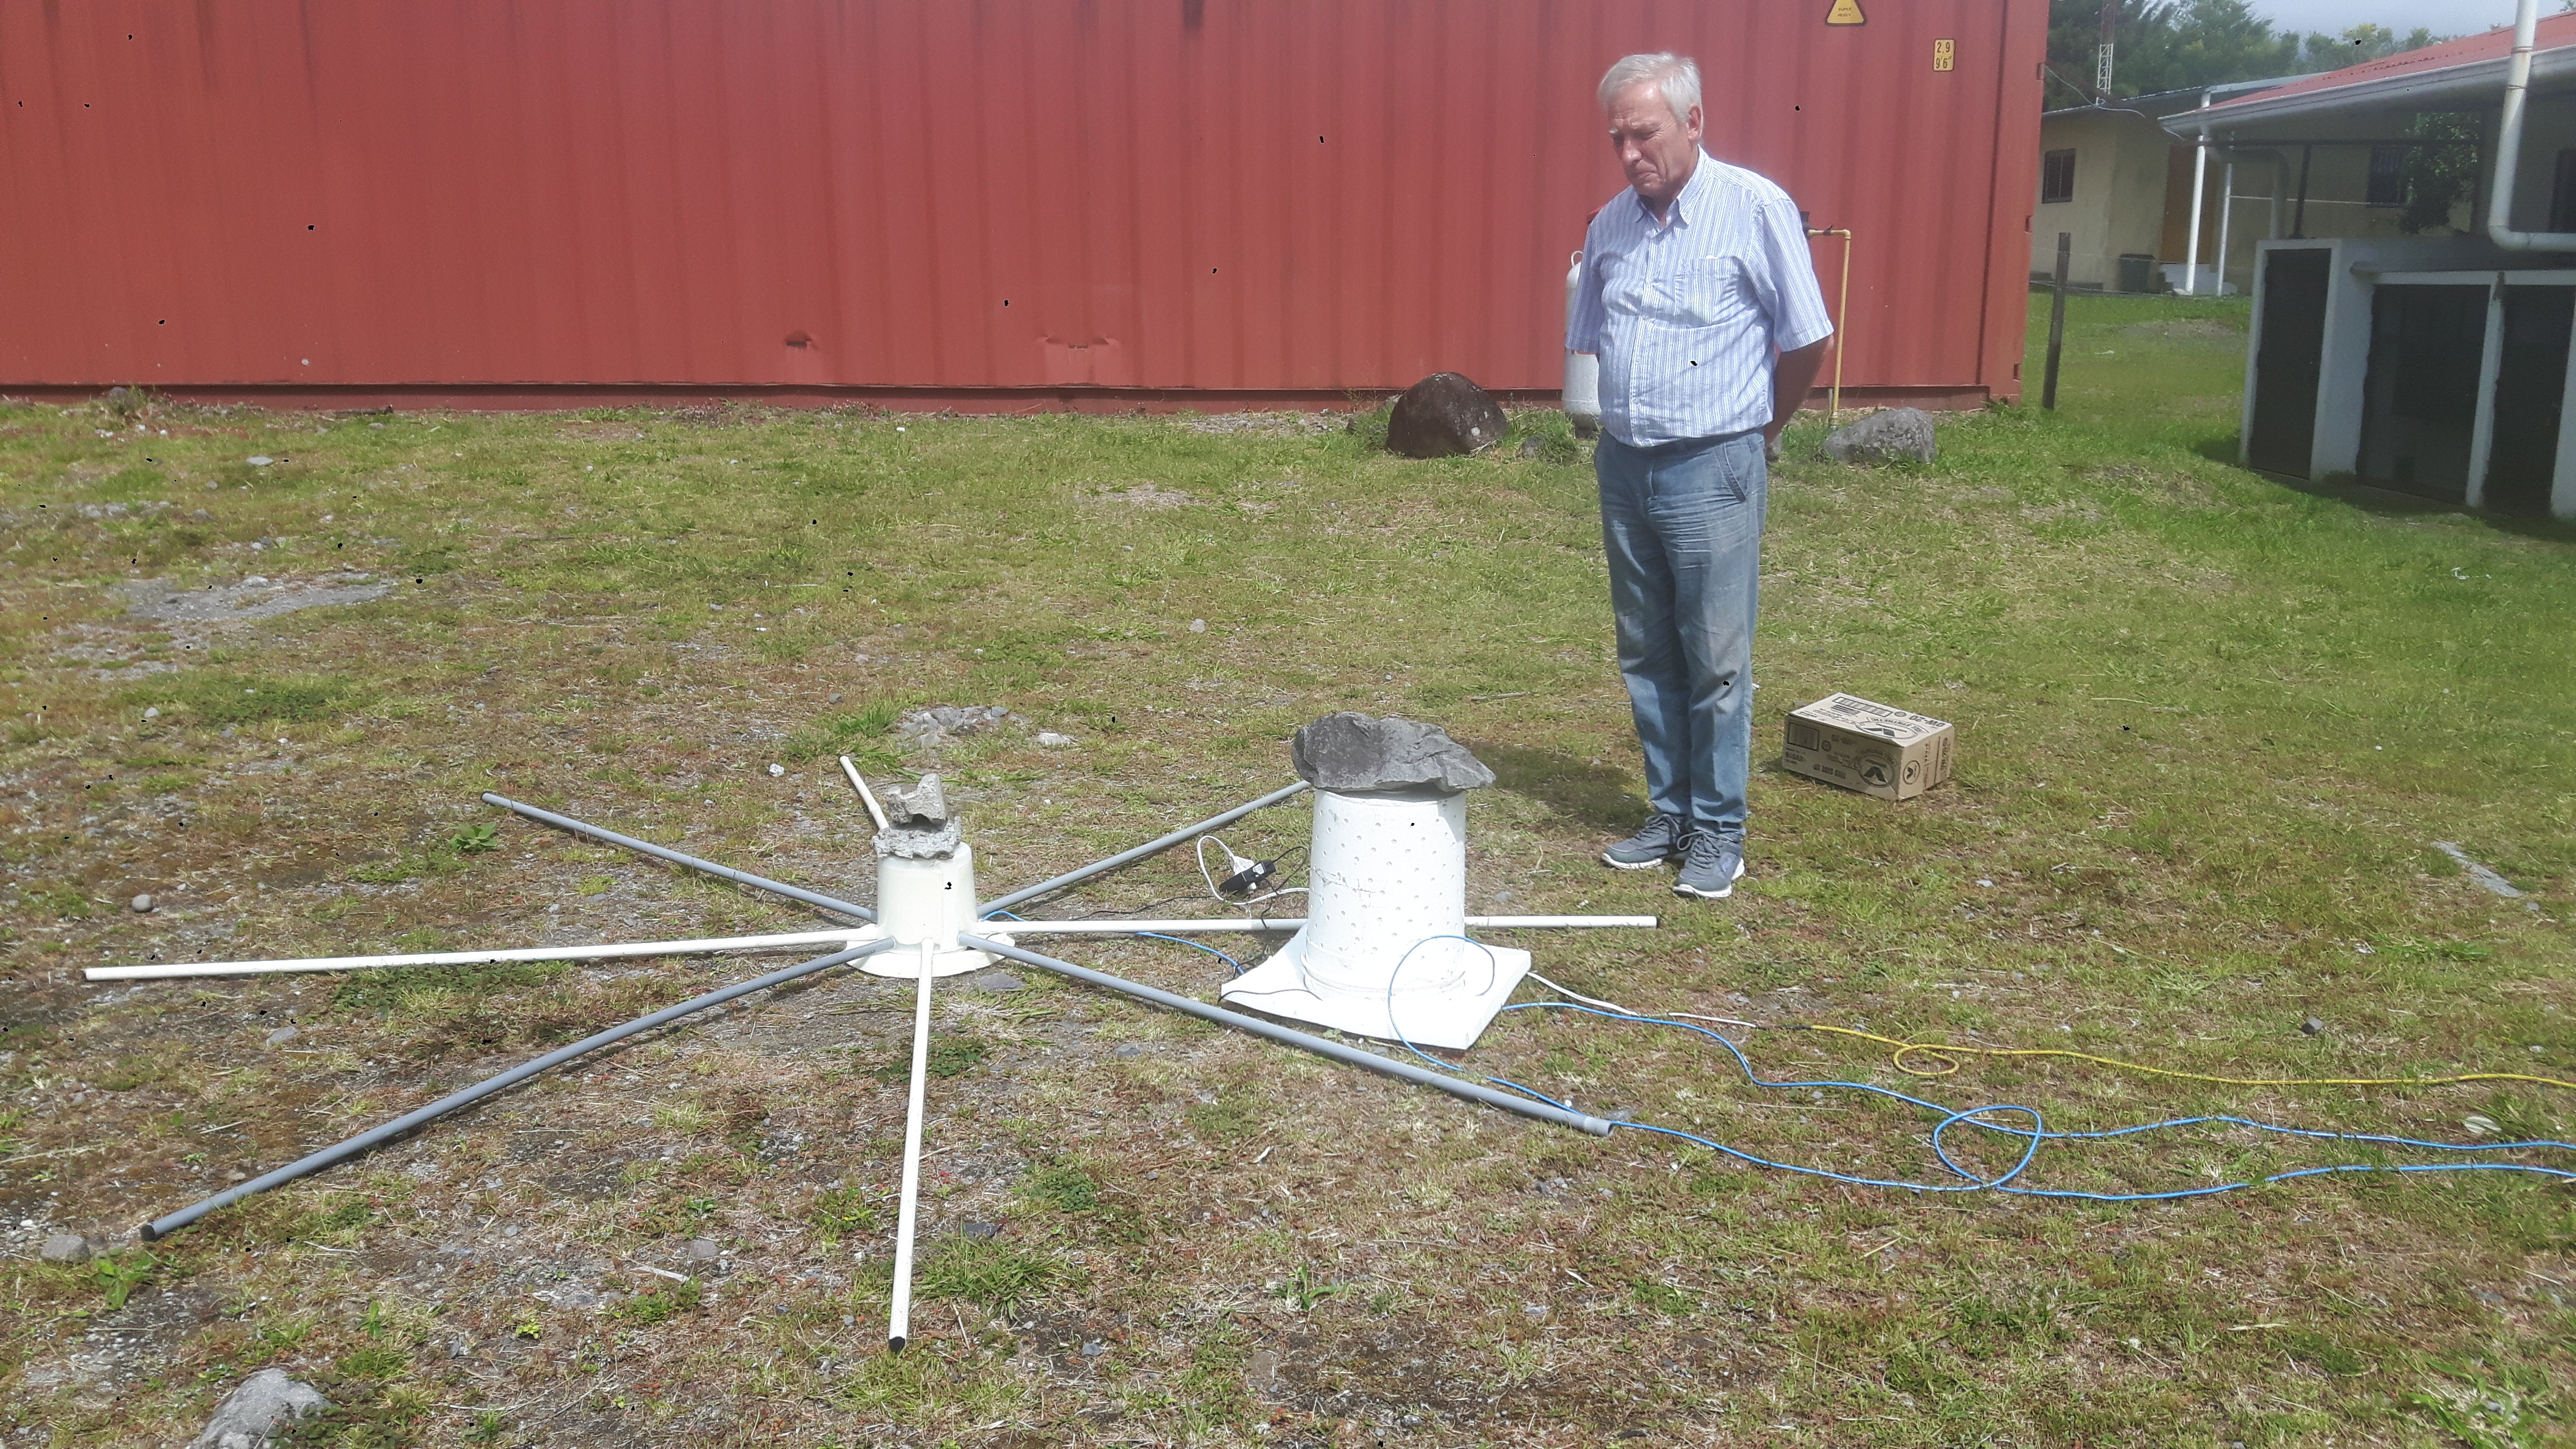
\includegraphics[width=\textwidth]{images/wind_infrasound.jpg}
	\end{center}
	\caption{
	Instação de um Raspberry Boom, uma inovação significativa no campo da monitoramento de infrassom. Tecnologia avançada e acessível ($\approx$ 1000 USD), que ofere uma maneira eficaz de detectar e analisar ondas sonoras de baixa frequência geradas por eventos naturais e antrópicos. Na foto observa-se um formato conhecido como \href{https://www.ctbto.org/our-work/monitoring-technologies/infrasound-monitoring}{pipe arrays}, empregado pela Organização do Tratado de Proibição Completa de Testes Nucleares (\href{https://www.ctbto.org/}{CTBTO}) para a supressão do ruído do vento nos dados.
    }
 \label{fig_wind}
\end{figure}

Observar ondas sonoras propagadas pelo ar é uma área crucial em diversos campos, desde a acústica e engenharia de som até a meteorologia e monitoramento ambiental. Essas ondas, resultantes de variações na pressão do ar, carregam uma riqueza de informações sobre fontes sonoras, características do ambiente e fenômenos naturais. Em resumo, a análise de ondas sonoras pelo ar é uma ferramenta poderosa e versátil que desempenha um papel vital em uma variedade de campos. Ao compreender como as ondas sonoras se comportam no ambiente atmosférico, podemos obter insights valiosos sobre uma ampla gama de fenômenos naturais e antrópicos, promovendo avanços significativos em diversas áreas das geociências.

\section{Tema: Monitoramento Infrassônico}

\subsection{Projeto: Instalação de estação de infrassom de baixo custo no Rio de Janeiro}

Uma variedade de fontes naturais e antropogênicas produzem ondas acústicas de muito baixa frequência (0,033 e 20 Hz), e devido a isso, pouca atenuação. Portanto, podem ser recebidas a centenas ou milhares de quilômetros de distância. Essas ondas acústicas de infrassom são detectados por sensores e redes de microbarômetros terrestres e originárias de fontes naturais e antrópicas (Grimmett et al., 2019). Fontes naturais de infrassom incluem terremotos, meteoros, vulcões, tsunamis, auroras e ondulações oceânicas; e as fontes antropogênicas são explosões nucleares atmosféricas e subterrâneas. O infrassom é uma tecnologia relativamente nova, quando comparada com estações sísmográficas e hidroacústicas, portanto a comunidade científica da área ainda bastante reduzida. No Rio de Janeiro, o \href{https://www.ctbto.org/our-work/international-monitoring-system}{Sistema de Monitoramento Internacional} da \href{https://funag.gov.br/biblioteca/download/934-Tratado_de_Proibicao_Completa_dos_Testes_Nucleares_CTBT.pdf}{Organização do Tratado de Proibição Completa de Testes Nucleares} possui uma estação que detecta e identifica partículas radioativas e gases nobres radioativos liberados na atmosfera provenientes de explosões nucleares no \href{https://www.gov.br/ird/pt-br/assuntos/noticias/noticias-2021/ird-sedia-estacao-de-monitoramento-global-capaz-de-detectar-materiais-radioativos-liberados-na-atmosfera}{Instituto de Radioproteção e Dosimetria}. A ideia deste projeto é inicialmente analisar e processar dados de infrassom, para a familiarização com esse tipo de dados. Posteriormente, este projeto visa a instalação de uma estação de baixo custo (\href{https://shop.raspberryshake.org/product/turnkey-iot-atmospheric-infrasound-monitor-rsboom/?attribute_pa_variation=indoor\&attribute_pa_license=private-use-125-discount}{$< 1000$ USD}), onde a unidade integra um geofone vertical e sensores de pressão omnidirecionais, juntamente com um digitalizador e um computador Raspberry Pi 3 em uma única caixa com dimensões de 135x110x70 mm. A principal motivação deste projeto é aumentar o número de cientistas utilizando estações de infrassom. O trabalho de Lamb et al. (2021) mostra que é possível utilizar esses sensores de baixo custo para recuperar sinais de infrassom com qualidade. Esses sensores de baixo custo são utilizados em vários trabalhos ao redor do globo, tendo utilizações na indústria e na academia, como podemos ver no \href{https://stationview.raspberryshake.org/}{mapa interativo} com as estações. 

\begin{fancyenum}{\faDatabase}{Banco de Dados}
	\item Dados de infrassom para teste no \href{https://www.ctbto.org/our-work/international-monitoring-system}{Sistema de Monitoramento Internacional}: \href{https://ds.iris.edu/gmap/\#network=IM\&planet=earth}{Incorporated Research Institution for Seismology} (\faUnlock);
\end{fancyenum}

\begin{fancyenum}{\faFutbol}{Objetivos}
	\item Analisar e caracterizar as atividades naturais, como terremotos e erupções vulcânicas, e atividades artificiais, como explosões nucleares e industriais, por meio da detecção de infrassons em dados de teste.
	\item Avaliar a possibilidade de instalação de uma estação de baixo custo no Rio de Janeiro;
	\item Realizar estudos sobre a Sismologia Urbana integrando dados de sensores de infrassom com estações sísmográficas.
\end{fancyenum}

\begin{fancyenum}{\faBrain}{Plano de Implementação}
	\item Associação destes eventos com as feiçõess batimétricas proeminentes que podem atuar como superfícies refletoras;
	\item O tempo de viagem entre o refletor e o sensor é previsto usando um modelo de velocidade do som oceânico dependente da estação;
	\item As chegadas diretas e refletidas são então usadas como entrada para o algoritmo de localização padrão, conforme descrito acima.
\end{fancyenum}

\begin{fancyenum}{\faShoppingCart}{Produtos}
	\item Melhoramento da cobertura azimutal da Rede Sismográfica Brasileira no mar;
	\item Melhorar a detecção e localização de grandes terremotos locais na Costa Brasileira.
\end{fancyenum}

\begin{fancyenum}{\faBook}{Bibliografia básica}
	\item Grimmett, D., Plate, R., Goad, J. (2019). Measuring Infrasound from the Maritime Environment. In: Le Pichon, A., Blanc, E., Hauchecorne, A. (eds) Infrasound Monitoring for Atmospheric Studies. Springer, Cham. https://doi.org/10.1007/978-3-319-75140-5;
	\item Lamb, O. D., Shore, M. J., Lees, J. M., Lee, S. J., \& Hensman, S. M. (2021). Assessing Raspberry Shake and Boom Sensors for Recording African Elephant Acoustic Vocalizations. Frontiers in Conservation Science, 1. doi:10.3389/fcosc.2020.630967.
\end{fancyenum}

%==============================================================================

\chapter{Financiamento dos projetos}
\label{cap_financiamento}

Tendo em mente que se eu lograr êxito e for aprovado para a vaga de pesquisador, estarei iniciando minha carreia, logo existe uma dificuldade para obter recursos para projetos autorais. Garantir recursos e financiamento é uma parte importante para garantir uma independência neste início de carreira. Os editais de fomento à pesquisa no Brasil estão cada vez mais competitivos e apenas projetos inovadores e com pesquisadores com um bom currículo são contemplados. Por isso, a minha proposta contempla projetos com metodologias recentes e inovadoras (Figura \ref{fig_resumo_projetos}), como exemplos da proposta temos o projeto de redução de ruído (capítulo \ref{cap_mar}) utilizando métodos de processamento de áudio e imagem em dados sísmicos e acústicos e a instalação de uma estação de infrassom de baixo custo (capítulo \ref{cap_ceu}) visando aumentar a interdisciplinaridade na instituição. A pesquisa requer colaborações entre diversos grupos de diferentes áreas para alcançar competitividade e fornecer respostas abrangentes às questões em pauta, por isso, a minha proposta abrange diversos ambientes, onde será possível ter a presença de colaboradores bem estabelecidos de diversas áreas. Isso não apenas fortalece uma proposta de financiamento de pesquisa, mas também amplia as chances de êxito. Como próximo passo, busco ter colaborações internacionais para aumentar o alcance das propostas.

\begin{figure}[ht]
	\centering
	\begin{tikzpicture}
	\pie{50/Ambiente marinho (4),
		37.5/Ambiente continental (3),
		12.5/Ambiente atmosférico (1)}
	\end{tikzpicture}
	\caption{Estatística da proposta de projetos em função dos diferentes ambientes de atuação.}
	\label{fig_resumo_projetos}
\end{figure}

No estágio pós-doutoral no Observatorio Nacional, vivenciei de perto o processo administrativo de grandes quantidades de recursos, entendendo os procedimentos burocráticos para a compra de equipamentos, fazer diferentes orçamentos, balanços e prestação de contas detalhada de todos os gastos, além de um relatório técnico detalhado das atividades, resutlados e produtos. SOmado a isso, participei da confecção de vários projetos de pesquisa, presenciei negativas e também aprovações. Creio que foi uma experiência sem igual para um jovem pesquisador, que assim que entrar na instituição terá que dividir seu tempo com treinamento de alunos novos, planejamento de aulas e direção de laboratório e participação em grupos internos de trabalho.




%==============================================================================

\chapter{Considerações Finais}
\label{cap_conclusao}

Este memorial narra minha jornada desde os meados dos anos 2000, quando iniciei meu curso de Geologia na Universidade Federal do Espírito Santo, até meu último estágio pós-doutoral no Observatório Nacional, instituição que desempenhou um papel fundamental ao longo da minha trajetória acadêmica. Durante meu último estágio pós-doutoral nessa instituição, pude aprofundar meu conhecimento e contribuir para projetos de pesquisa de grande relevância. Nessa maratona acadêmica, passei por 4 instituições federais em 4 estados diferentes, visitei 15 estados para participar de conferências nacionais e aulas de campo e visitei 5 países assistindo a cursos e conferências internacionais graças ás oportunidades geradas pelos programas de pós-graduação, projetos e bolsas que estive envolvidos.

Os números apresentados acima, assim como a lista \ref{lista_divulgacao}, fornecem uma visão detalhada dessa abordagem multifacetada na popularização da ciência e das atividades do Obseravtório Nacional ao longo do período que estive na instituição, um total de 38 atividades ao longo de 3 anos. Destaco que concedi dezenas de entrevistas, totalizando 24 (13 escritas, 8 gravadas e 3 ao vivo), contribuí revisando textos na temática da Sismologia e Geologia que foram publicados nas redes sociais do Obseravtório Nacional. Além disso, fiz parte da comitiva que participou do \href{https://www.gov.br/observatorio/pt-br/assuntos/areas-de-atuacao/divulgacao-e-popularizacao-da-ciencia/on-riw}{Rio Innovation Week}, o maior evento de tecnologia e inovação da América Latina, para apresentar as iniciativas, ações e projetos ligados ao \href{https://www.gov.br/mcti/pt-br}{MCTI}. Somada a isso, ministrei dois minicursos em duas instituições de ensino superior, na Universidade Federal do Espírito Santo para o curso de Geologia na \href{https://www.instagram.com/segeo.ufes/}{Semana de Estudos Geológicos da Universidade Federal do Espírito Santo} e no Instituto de Física da Universidade Federal de Pernambuco na \href{https://www.gov.br/observatorio/pt-br/assuntos/noticias/i-escola-itinerante-da-geofisica-do-observatorio-nacional-e-realizada-na-ufpe}{I Escola Itinerante da Geofísica do Observatório Nacional}. Ministrar um curso em outras instituições, não apenas promove a disseminação do conhecimento especializado, mas também desempenha um papel crucial na visibilidade e reputação do Observatório Nacional. Esses eventos compartilham expertise em contextos acadêmicos diversos, estabelecendo laços colaborativos e fortalecendo a presença no cenário acadêmico. Além disso, o envolvimento em eventos externos fortalece parcerias e colabora para o crescimento do programa de iniciação científica e pós-graduação do ON, estimulando a atração de novos alunos.

Atuo em diversas linhas de pesquisa relacionadas a Sismologia, com aplicações na indústria e na academia. Toda a minha caminhada estive envolvido à tópicos da Sismologia, no entanto, sempre estive aberto a coloborar com outras áreas. A experiência na Sismologia Marinha mostrou minha habilidade multidisciplinar com outras áreas da Ciências Marinhas. Todo o ensino superior, de alta qualidade, foi-me proporcionado de forma gratuita e através de inúmeros auxílios para estudos na pós-graduação. Se houver a possibilidade, estou pronto para retribuir com a experiência que adquiri em pesquisa, ensino e divulgação científica. Caso tenha a oportunidade, pretendo buscar colaborações com os pesquisadores e pesquisadoras do Observatório Nacional e de outras instituições na região Sudeste, no Brasil e  na América do Sul, inicialmente. Posteriormente, a vontade é de consolidar colaborações com outras regiões do mundo. As áreas de atuação são diversas, como estrutura da Terra, regionalmente e globalmnte, monitoramento sísmico e acústico, tectônica e de instrumentação geofísica. No quesito do ensino, eu tenho a capacidade de ajudar a pós-graduação em diversos tópicos que ligam a Geologia, Geofísica e Sismologia, propondo disciplinas eletivas, cursos de aperfeiçoamento e cursos de curta duração. Além disso, atualmente existe a expansão da utilização de ferramentas remotas para o ensino, aperfeiçoamento e divulgação da Ciência. 

Desde os dias de estudante de graduação até o estágio pós-doutoral no Observatório Nacional, tenho vivenciado uma jornada repleta de descobertas, desafios, derrotas e conquistas, que não só moldaram minha carreira acadêmica, mas também ampliaram minha visão de mundo e fortaleceram meu compromisso com a excelência na pesquisa e inovação científica. Além de todo o conhecimento técnico acumulado durante minha trajetória acadêmica, o maior benefício adquirido foi a independência acadêmica. Isso não significa que eu não necessito da ajuda de ninguém ou posso seguir e realizar completamente sozinho os projetos e atividades propostos. O que quero dizer é que eu passei a desenhar de forma clara o que eu precisava estudar mais e quais eram as minhas principais limitações e traçar o caminho para lograr êxito em cada caminhada. Em suma, seria uma honra ter a oportunidade de contribuir para a instituição, tanto na formação de novos talentos quanto na condução de pesquisas de inovadoras.

\end{document}
